\documentclass[11pt]{article}
\usepackage{cs1200}
\usepackage{tikz}
\usepackage{chessboard}
\usepackage{xcolor}

\begin{document}

\psHeader{5}{Wed Oct. 22, 2025 (11:59pm)}

Please see the syllabus for the full collaboration and generative AI policy, as well as information on grading, late days, and revisions.

All sources of ideas, including (but not restricted to) any collaborators, AI tools, people outside of the course, websites, ARC tutors, and textbooks other than Hesterberg--Vadhan must be listed on your submitted homework along with a brief description of how they influenced your work. You need not cite core course resources, which are lectures, the Hesterberg--Vadhan textbook, sections, SREs, problem sets and solutions sets from earlier in the semester. If you use any concepts, terminology, or problem-solving approaches not covered in the course material by that point in the semester, you must describe the source of that idea. If you credit an AI tool for a particular idea, then you should also provide a primary source that corroborates it. Github Copilot and similar tools should be turned off when working on programming assignments.

If you did not have any collaborators or external resources, please write 'none.' Please remember to select pages when you submit on Gradescope. A problem set on the border between two letter grades cannot be rounded up if pages are not selected. 

\vspace{1em}

\textbf{Your name: }

\textbf{Collaborators and External Resources:}

\textbf{No. of late days used on previous psets: }

\textbf{No. of late days used after including this pset: }



\begin{enumerate}
   \item  (Rotating Walks)  
    Suppose we are given $k$ digraphs on the same vertex set, $G_0=(V,E_0), G_1=(V,E_1), \ldots, G_{k-1}=(V,E_{k-1})$.  For vertices $s,t\in V$, a {\em rotating walk} with respect to $G_0,\ldots,G_{k-1}$ from $s$ to $t$ is a sequence of vertices $v_0,v_1,\ldots,v_{\ell}$ such that $v_0=s$, $v_\ell=t$, and $(v_i,v_{i+1})\in E_{i \bmod k}$ for $i=0,\ldots,\ell-1$.  That is, we are looking for walks that rotate between the digraphs $G_0,G_1,\ldots,G_{k-1}$ in the edges used.
    \begin{enumerate}
        \item Show that the problem of finding a \ShortestRotatingWalk\ from $s$ to $t$ with respect to $G_0,\ldots,G_{k-1}$ 
        can be reduced to \SingleSourceShortestPaths\ via a reduction that makes one oracle call on 
        a digraph $G'$ with $kn$ vertices and $m_0+m_1+\cdots+m_{k-1}$ edges, where $n=|V|$ and $m_i=|E_i|$.
        We encourage you to index the vertices of $G'$ by pairs $(v,j)$ where $v\in V$ and $j\in [k]$. 
        Analyze the running time of your reduction and deduce that \ShortestRotatingWalk\ can be solved in time $O(kn+m_0+\cdots+m_{k-1})$, and provide a proof of correctness.
        \label{part:ReduceToOrdinary}  To test your reduction and algorithm, try running through the example in Part~\ref{part:BFS}.


        

        
        


        \item \label{part:BFS} 
   
        Run your algorithm from Part~\ref{part:ReduceToOrdinary} (by hand; no programming necessary) on the following pair of graphs $G_0$ and $G_1$ to find the shortest rotating walk from $s=a$ to $t=c$; this will involve solving \SingleSourceShortestPaths\ on a digraph $G'$ with $2\cdot 7=14$ vertices. Fill out the table provided below with the BFS frontier in $G'$ at each iteration, labelling the vertices of $G'$ as $(a, 0),(b, 0),\ldots,(g,0),(a,1),(b,1),\ldots,(g,1)$, and for each vertex $v$ in the table, drawing an arrow in the graph from $v$'s BFS predecessor to $v$. 


            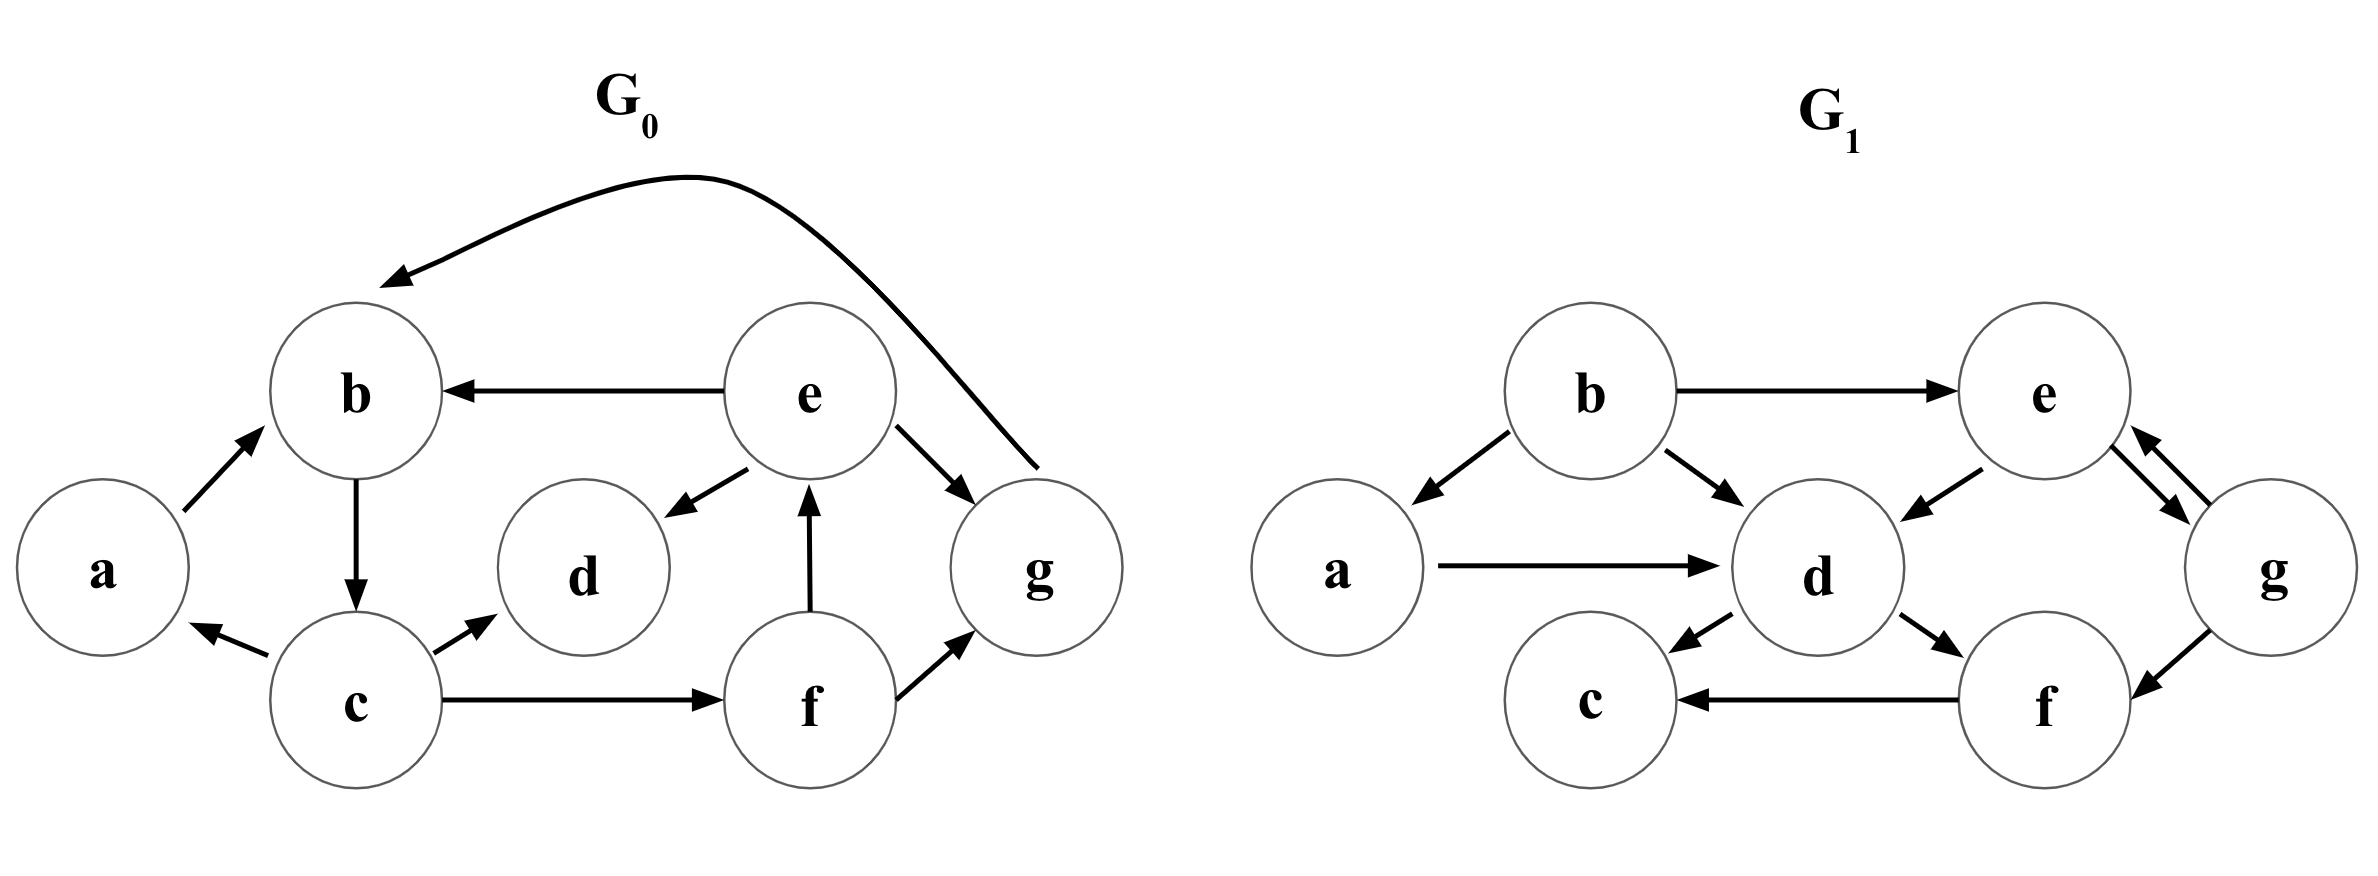
\includegraphics[width=14cm]{ps5_graph.png}

            \begin{table}[ht]
        \centering
        \begin{tabular}{c|c|c}
            $d$ & Frontier $F_d$& Predecessor Relationships \\
            \hline
              0 &  & \\
              1 &  & \\
              2 &  & \\
              3 &  & \\
              4 &  & \\
        \end{tabular}
        \end{table}




    
    \item 
        A group of three friends decides to play a new cooperative game (similar to the real-life board game Magic Maze).  They rotate turns moving a shared single piece on an $n\times n$ grid.  The piece starts in the lower-left corner, and their goal is to get the piece to the upper-right corner in as few turns as possible.  Many of the spaces on the grid have visible bombs, so they cannot move their piece to those spaces.  Each player is restricted in how they can move the piece.  Player 0 can move it like a chess rook (any number of spaces vertically or horizontally, provided it does not cross any bomb spaces). Player 1 can move it like a chess bishop (any number of spaces diagonally in any direction, provided it does not cross any bomb spaces).  Player 2 can move it like a chess knight (move to any non-bomb space that is two steps away in a horizontal direction and one step away in a vertical direction or vice-versa).   Using Part~\ref{part:ReduceToOrdinary}, show that given the $n\times n$ game board (i.e., the locations of all the bomb spaces), they can find the quickest solution in time $O(n^3)$.  
        (Hint: give a reduction, mapping the given grid to an appropriate instance $(G_0,G_1,\ldots,G_{k-1},s,t)$ of Shortest Rotating Walks. No proof of correctness necessary, but you must specify runtime.)


 



 \end{enumerate}

  \item (Reductions Between Variants of \IndependentSet) 
 Consider the following three variants of the IndependentSet problem:
 \begin{itemize}
     \item \IndependentSetOptimizationSearch: given a graph $G$, find the largest independent set in $G$.
     \item \IndependentSetThresholdSearch: given a graph $G$ and a number $k\in \N$, find an independent set of size at least $k$ in $G$ (if one exists).
     \item \IndependentSetThresholdDecision: given a graph $G$ and a number $k\in \N$, decide (by outputting YES or NO) whether or not there is an independent set of size at least $k$ in $G$. 
 \end{itemize}

 \begin{enumerate}
 \item Suppose that there is an algorithm running in time $T(n,m)\geq n+m$ that solves \IndependentSetOptimizationSearch\ on graphs with at most $n$ vertices and at most $m$ edges.  Prove that there is an algorithm running in time $O(T(n,m))$ that solves \IndependentSetThresholdDecision. Be sure to both prove correctness and analyze runtime for the algorithm you provide.


 
  
 
 \item Suppose that there is an algorithm running in time $T(n,m)\geq n+m$ that solves \IndependentSetThresholdSearch\ on graphs with at most $n$ vertices and at most $m$ edges.  Prove that there is an algorithm running in time $O((\log n)\cdot T(n,m))$ that solves \IndependentSetOptimizationSearch.  (Hint: Come up with a reduction that makes at most $\log n$ oracle calls.  You might find it useful to first find one that makes at most $n$ oracle calls.) You do not need to prove correctness for your algorithm, but do analyze its runtime.




 
 
  \item Suppose that there is an algorithm 
 running in time $T(n,m)\geq n+m$ that solves \IndependentSetThresholdDecision.   Prove that there is an algorithm running in time $O(n\cdot T(n,m))$ that solves \IndependentSetThresholdSearch.
(Hint: Show that $G$ has an independent set of size at least $k$ containing vertex $v$ iff $G-N(v)$ has an independent set of size at least $k-1$, where $G-N(v)$ denotes the graph obtained by removing $v$ and all of its neighbors from $G$.  Use this fact and the oracle to determine for each vertex $v$, whether or not to include $v$ in the independent set.  Remember to update the graph appropriately after each decision.) Be sure to both prove correctness and analyze runtime for the algorithm you provide.




\end{enumerate}
 We remark (but you don't need to submit anything) that the combination of the three previous problem parts means that for every constant $c\in [1,2]$, if there is an algorithm solving any one of the three problems in time $(n+m)^{O(1)}\cdot c^n$, there are algorithms solving the other two problems in $(n+m)^{O(1)}\cdot c^n$ time.  The best known algorithm (by Xiao and Nagamochi, 2013) has $c \approx 1.1996$.
 



\item (Reflection) Take one homework problem you have worked on this semester that you struggled to understand and solve, and explain how the struggle itself was valuable.  In the context of this question, describe the struggle and how you overcame the struggle. You might also discuss whether struggling built aspects of character in you (e.g. endurance, self-confidence, competence to solve new problems) and how these virtues might benefit you in later ventures. 

\item Once you're done with this problem set, please fill out \href{https://forms.gle/D7d6EuQVCnTmz8ku6}{this survey} so that we can gather students' thoughts on the problem set, and the class in general. It's not required, but we really appreciate all responses! \textbf{This week would be a great time to provide any mid-semester feedback, which could help us improve the course in the second half of the semester.}


  \end{enumerate}






\end{document}
